\documentclass[conference,compsoc]{IEEEtran}
%\ifCLASSOPTIONcompsoc
  %% IEEE Computer Society needs nocompress option
  % requires cite.sty v4.0 or later (November 2003)
  %\usepackage[nocompress]{cite}
%\else
  % normal IEEE
  \usepackage{cite}
%\fi
\usepackage{graphicx}
\usepackage{float}
\graphicspath{{C:/Users/NEGU/Desktop/Parallel-Image-FIltering/report/images/}}
\usepackage{amsmath}
\newcommand{\Mod}[1]{\ (\text{mod}\ #1)}
% correct bad hyphenation here
\hyphenation{op-tical net-works semi-conduc-tor}

\begin{document}

\title{Speed Up of Image Filtering using Parallel Programming Models}
% author names and affiliations
\author{\IEEEauthorblockN{Jos\'{e} Agust\'{i}n Barrachina}
\IEEEauthorblockA{IEEE Student Member\\
\'{E}cole Polytechnique\\
Universit\'{e} Paris-Saclay\\
Route de Saclay, 91128 Palaiseau, France\\
Email: joseagustin.barra@gmail.com}
\and
\IEEEauthorblockN{Fran\c{c}ois Bidet}
\IEEEauthorblockA{\'{E}cole Polytechnique\\
Universit\'{e} Paris-Saclay\\
Route de Saclay, 91128 Palaiseau, France\\
Email: francois.bidet@polytechnique.edu}}

% make the title area
\maketitle

\begin{abstract}
The aim of this project was to speed-up a target application through multiple parallelism models (MPI, OpenMP and CUDA) for various architectures (CPU and GPU) and conclude which approach is the most suitable for the specific application. 
\end{abstract}
\IEEEpeerreviewmaketitle

\section{Introduction}
A base C/C++ code that implements an image filtering was given. The aim of this work is to optimize the operation time of the code by using parallel programming methods such as MPI, OpenMP and CUDA.
The base C/C++ code covers a large spectrum of algorithms in HPC and Big Data. The Image Filtering can be seen as a direct application of Big Data programs. This application uses a stencil-based scheme to apply a filter to an existing image or set of images. It means the main process of this code is a traversal of each pixel of the image and the application of a 2D stencil \cite{CoursePage}.

We will work with GIF image because this format has the following advantages:
\begin{description}
	\item[$\bullet$] Easy to manipulate
	\item[$\bullet$] Widespread format (social networks)
	\item[$\bullet$] Allow animation (multiple images). which can be paralized as well.
\end{description}

\subsection{Project Organization} \label{sec:project-organization}
This project was done using github version control repository. Each different strategy of parallelizing was made in a different branch, having as master branch the original serial program. So that in the end a merge was done with the strategies that proved to work better.

The different branches are as follows:
\begin{description}
	\item[$\bullet$] \textbf{Master} Contains the file with the sequential code.
	\item[$\bullet$] \textbf{Result} Contains the final realization with a combination of CUDA, MPI and OpenMP. Section: \ref{sec:results}
	\item[$\bullet$] \textbf{MPI\_over\_images\_of\_gif} Applies MPI to treat each image of a gif separatelly. Section: \ref{sec:treating-each-image-sep}
	\item[$\bullet$] \textbf{Bidouille} Applies MPI to divide the work on each image. Section: \ref{sec:treating_subparts}
	\item[$\bullet$] \textbf{OpenMP\_divide\_image} Applies OpenMP to divide the work on each image. Section: \ref{sec:OpenMP}
	\item[$\bullet$] \textbf{CUDA\_filtering} Applies CUDA to divide the work on each image. Section: \ref{sec:CUDA}
\end{description}

% Add references to the bulletpoints in there

\subsection{Testing Work}
To test the efficiency of the program, many files were created. A simple C program was done to make a summary of all the results obtained. This summary is only an addition of the time taken to apply the filter to each gif image.

%TODO: here write about the coefficent test/bash we made. We can put a name to this coefficient to reference it later when explaining the resutls. Something like "expected improvement time coefficient" that will literally be the expected improvement of the gif filtering without knowing anything about the image.

Also, a shell file was created to run many gif images one after the other. Various variations of this shell were made to run the test only on gif files that share some property as for example, containing only one image or on the contrary containing more than one image.

With the help of ImageMagik \cite{IMAGEMAGICK}. Two shell files were created to compare the original (serial) program output with the new parallel optimized program in order to check that it works perfectly. The first bash file creates a output image that, if both images are exactly the same, should create a complete black image. Because this method can be difficult to be sure the images are exactly the same, a second bash file was created that compares pixel by pixel each image and output 0 if the image is completely identical. In that case, the first file is used to check if the images are identical and if they are not, the second bash can be used to see what the mistake is.

\section{Image Filtering Program}
This topic focuses on a specific image filter that is useful to detect objects and edges inside various images. This filter is called Sobel and it applies on a greyscale image. Therefore, the first step is to transform the image from a color one to a set of gray pixels. 

Then, a blur filter is applied to a small part of the images to exclude the borders. Thus, the main goal is to parallelize an application that apply multiple filters (grayscale, blur and Sobel) to a GIF Image (either a single image or an animated gif). \cite{CoursePage}
\subsection{Structure}
The algorithm can be divided into three main parts:
\begin{description}
	\item[1$\cdot$] GIF import (section \ref{sec:GIF-import})
	\item[2$\cdot$] SOBEL filter (section \ref{sec:SOBEL-filter})
	\item[3$\cdot$] Export image (section \ref{sec:Export-image})
\end{description}
A main function already measures and output the time taken by each of the three listed parts of the project.

\subsubsection{GIF import}\label{sec:GIF-import}
This part just load the gif file into a pixel array. 

\subsubsection{SOBEL filter}\label{sec:SOBEL-filter}
This part of the code applies actually three different filters:
\begin{description}
	\item[1$\cdot$] \textbf{Gray Filter} Convert the pixels into a grayscale
	\item[2$\cdot$] \textbf{Blur Filter} Apply blur filter with convergence value
	\item[3$\cdot$] \textbf{Sobel Filter} Apply Sobel filter on pixels
\end{description}

\subsubsection{Export image}\label{sec:Export-image}
This is just the inverse of the first part (section \ref{sec:GIF-import}). Converts the array of pixels and creates a gif file which is then stored into a folder.

\section{Parallel Optimization Languages}
\subsection{MPI} \label{sec:MPI}
MPI stands for Message Passing Interface, is a standardized and portable message-passing system to function on a wide variety of parallel computing architectures. MPI takes each worker as a process and standardizes the message passing operation between them.
\subsubsection{Treating each gif image separately} \label{sec:treating-each-image-sep}
Each gif image can have several images saved together, the core of this optimization method was to make each worker to treat each image separately in order to make the process faster.
Two different ways of organizing the work distribution can be applied:
\begin{enumerate}
	\item Static Work Distribution
	\item Dynamic Work Distribution
\end{enumerate}
In the first case, the Static Work Distribution just gives each worker a different but precomputed image. For example, should there be "n" images and "P" processes, we can make a rule that follows the following equation:
\begin{equation}
task \equiv n \mod P
\end{equation} 
Where task will be the number of the process that must work on the image number \textit{n}. In this case, each process will work in their precomputed images and they will be always the same in each run of the code no matter how much time each process takes with each image.

In the case of the dynamic distribution, an initial work (in this case image) is given to each thread, the first one to finish will be given the next work (next image). It is important to notice that in order to manage this distribution, one thread must be used and so it will not be able to do the computation, this is called overhead. For example, if there are three workers and three images, one worker will give the first two images to the remaining two workers, and the first of them to finish will be given the next image to work on.

Both strategies may be useful depending on some variables. For example, if the different images inside the gif file are very different from each other, it may be possible that using dynamic work distribution will make the most of the resources.
If the nodes or threads have very different computation power, for example, they are run in different computers with very different processors and specifications, then dynamic work distribution may also be more effective in this case.
Both cases named before are based that the time each threads takes to work is very different from each other, the more difference there is with each thread execution time, the more effective it will be to use dynamic work distribution. If, on the other hand, the computational power of the threads are similar and all the images of a gif image are similar so that is not expected that each thread will take a great difference of time to make the computation, then it in necessary to look for other variables that may make a difference between each method.

The negative impact of the dynamic work case will be dependent on the amount of tasks used for the computation. With three MPI threads, the loss of one task will make a great negative impact as there will be only two tasks to work on each image instead of three. To go to extremes, with only two tasks, applying dynamic distribution will result in a serial work and no optimization will be done. The more MPI tasks are used, the less impact the overhead will have over the code. As a general rule, the less MPI tasks, more convenient it will be to use static work distribution, whereas the more MPI task, better for dynamic distribution as long as there are no more tasks than images of the gif. Should there be more (at least one) MPI tasks than images of the gif file, then the loss of one task to manage the work distribution will not affect the general performance of the code and there will be no relevant difference between both work distributions as each task will manage one image while others will not be used.

The final decision will be a trade off between the difference of time each task takes to do the job and the amount of available tasks, taking also into account the number of images in the gif file to be filtered. This variables however cannot be known for sure beforehand as the intention is to optimize the work for any gif image in general.

It was chosen to make a Static no only because it was an easier implementation, but also because gif images are supposed to have all images similar to each other. Also, each node is supposed to be run at least for our case in similar hardware, for that reason, the time taken by each process to filter each image will be almost the same, and using a dynamic distribution won't be of much help. 
Also, all the remaining MPI tasks can be used to speed up the computation time treating each image as explained on section \ref{sec:treating_subparts} so that the more MPI tasks I have the better.
Of course, this approach will not be so should each image of the gif file be very different to each other.

%added by Kujyto
%begin of Kujyto's part
\subsubsection{Treating subparts of each image} \label{sec:treating_subparts}
A master task splits the input images in subpart and sends each subpart to a slave task, which compute the blur filter.
After the work, the master task merges each part of the original image and finishes the blur filter iteration.

This work can be done as long as the difference between the input image and the blured image is bigger than a predefined threshold.

The biggest problem of this solution is to split the input image in subparts with a overlap area.

We get the best reduction of time with 8 tasks on the same node than any number of tasks on many node because communications between nodes are much slower than in the same node.
%end of Kujyto's part

\subsubsection{Results}
When using MPI to treat each image of the gif by each task, there was no increase on performance when the gif has only one image as expected. 

The test was run over seven different gif files that contain more than one image each. The average time to apply for example the blur filter with the original sequential program was 8.1 seconds. This time could be taken down to a minimum of 1.1 seconds. Values were between that range depending on how many MPI tasks were chosen.

Running this code in a gif with 20 high resolution images, the blur filter time was taken down from 4 seconds to 0.4 seconds, which means that the MPI code takes 10\% of the time the sequential filter uses. Using more than 20 tasks takes almost the same time as 20 which is expected as the tasks 21 and higher will not work at all and will only consume communication time.
The loading of the image however, was not so much improved, taken the time from 0.36 to 0.3 seconds.

% TODO: see the coefficient result. Say that the gther is done only in the end.

% TODO: write something about your performance Fran

\subsection{OpenMP} \label{sec:OpenMP}
OpenMP stands for Open Multi-Processing. It is an application programming interface (API) that supports milti-platform shared memory multiprocessing programming in C, C++ and Fortran on most platforms, processor architectures and operating systems.
OpenMP provides a portable, scalable model for developers of shared memory parallel applications.
It consist of a set of three primary API components:
\begin{description}
	\item[1$\cdot$] Compiler Directives
	\item[2$\cdot$] Runtime Library Routines
	\item[3$\cdot$] Environmental Variables
\end{description}

OpenMP comes included in gcc compiler so that only a flag is needed for gcc to compile the Parallel code made with OpenMP.

\subsubsection{Treating subparts of each image}
As in \ref{sec:treating_subparts}, the goal of this part was to implement a program that divides the image into sections and each thread treats each section. The approach was different than on the MPI implementation. Here, it was not the main which was treated but every specific filter function.

\subsubsection{Results} \label{sec:results}
The results were quite effective. Running the algorithm through many different gif images, the Blur Filter Time was reduced by around 75\% . The Sobel Filter Time was reduced around 60\% and the Gray Filter was reduced a 30\%. This results are taken by adding all the different times together and comparing both results of the original program and the OpenMP implementation.

\subsection{CUDA}\label{sec:CUDA}

\subsection{CUDA vs OpenMP}

%TODO: make test in Result with the both codes and see wich one works better.

\section{Final program}

Figure \ref{fig:Git-Project-Flow-Diagram} shows the sequential work of the project representing the creation and merging of each branch discussed previously on section \ref{sec:project-organization}. The left part of the graph represent an early period in time while the right part is the completion of the actual project code.

\begin{figure}[H]
	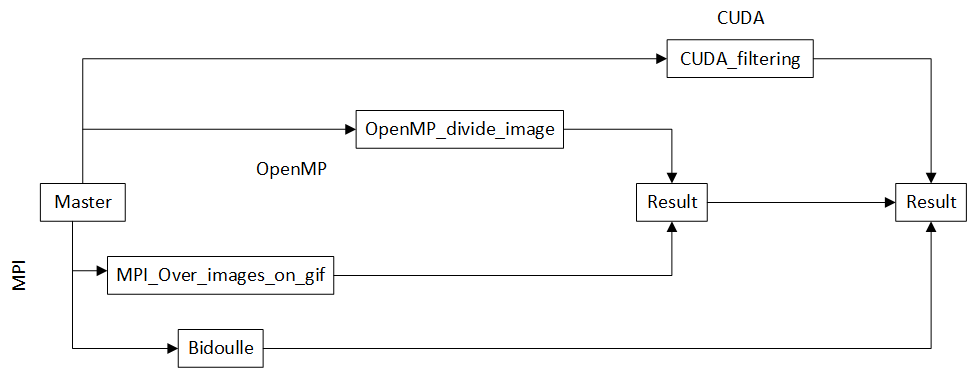
\includegraphics[width=7cm]{GitDiagram.png}	\centering
	\caption{Git Project Flow Diagram	\label{fig:Git-Project-Flow-Diagram}}
\end{figure}

As it can be seen in the figure, the first approach was to implement the MPI code with both strategies discussed on \ref{sec:MPI}. The MPI part over each image separately took less time because of less complexity and as soon as it was ready, the OpenMP (\ref{sec:OpenMP}) code was implemented. As soon as this OpenMP was ready, it was merged with the MPI part. In this merge, MPI treated each image in each different node while OpenMP divides the work for that image within each core. This method had two inconveniences, first of all, should the gif file have less images that the MPI threads, some of those threads will be unused. Also, the GPU is not used at all to help in the optimization process.

When running the sequential code, the blur part takes around 70\% of the time. For that reason, the blur filter was taken as a priority and the optimization methods were focused on this part alone. The following explanation of the code was only done for the blur filter, which means that outside the blur filter, the final code works as recently explained.

Before continuing with the explanation of the final code, it will be important to pay attention to the hardware itself. There are a number of computers (nodes), each with it's own CPU and GPU. Only MPI can be used to take advantage of each node so it was used to do exactly that. MPI was used to take advantage of any number of nodes or computers possible. Because it was the aim of the project to try to apply as many languages as possible, MPI was not used or intended to be used to run on the different CPU cores, OpenMP was used for this purpose, which actually obtained better results than MPI, probably because the communication between threads is done in a more efficient way automatically by the compiler. This will be important to understand so that MPI is not run with many processes in the same node. Should that happen, the threads made by MPI within one node will "fight" for the resources inside the computer and will result in a loss of efficiency, although the code should work anyway.

The MPI application was made by a combination of both sections \ref{sec:treating-each-image-sep} and \ref{sec:treating_subparts}. First, MPI uses each thread to work on each image of the gif. Should the threads be more than needed, sub-groups will be created to treat each image with the technique explained in section  \ref{sec:treating_subparts}. If a gif image has for example 2 images, and three nodes are used, then node 0 and 2 will be used to treat the first image while node 1 will work with the second image alone.

This application of both techniques of MPI, however, was only applied to the blur filter alone for the reason stated before. On the blur filter, another step was added. The use of the GPU to make the processing.

\begin{figure}[H]
	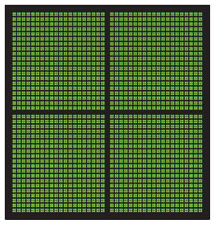
\includegraphics[width=5cm]{gpu.png}	\centering
	\caption{GPU Architecture \label{fig:GPU-Architecture}}
\end{figure}

The CUDA kernel was done with a three dimensional block, a two dimensional block for the image itself to make it easy to compute the row and column of the treated image and a third dimension was added to treat each RGB (Red Green Blue) color. In order to make use of the multiprocessors, a two dimensional grid was made as shown in \ref{fig:GPU-Architecture}. In such figure one color architecture is shown. A 2x2 grid is represented with a two dimensional size blocks which corresponds to one of the three colors. Each small green square of the image is a thread or (in the best case scenatio) a GPU core. The row and column of the image to be filtered is a combination of the grid and block index. Whereas the color is given by the z index of each block.

The blur filter makes use of the CUDA kernel to process each image as explained on \ref{sec:CUDA}. It is important to remark that as it was said before, running many MPI threads in one node will make one thread have to wait till the other thread finish using the GPU and will affect the final performance.

\section{Conclusion}

% use section* for acknowledgment
\ifCLASSOPTIONcompsoc
  % The Computer Society usually uses the plural form
  \section*{Acknowledgments}
\else
  % regular IEEE prefers the singular form
  \section*{Acknowledgment}
\fi

%TODO: add all the CUDA bibliography
\newpage
\IEEEtriggeratref{8}
\bibliographystyle{IEEEtran}
\bibliography{ref}

\end{document}


